% Problemstellung / Motivation
%   vielleicht ein Beispiel, wenn ihr wollt
% Eure Lösung: Balanced Banana
%   Wie löst es die Problemstellung / was tut es?
%   Wie funktioniert es? (nutzt die Grafiken aus eurem Pflichtenheft)
%   Nennenswerte Features

\documentclass{beamer}

\usepackage[utf8]{inputenc} % use utf8 file encoding for TeX sources
\usepackage[T1]{fontenc} % avoid garbled Unicode text in pdf
\usepackage[german]{babel} % german hyphenation, quotes, etc
\usepackage{hyperref} % detailed hyperlink/pdf configuration
\hypersetup{ % `texdoc hyperref` for options
pdftitle={Pflichtenheft Balanced Banana},
bookmarks=true,
}
\usepackage{csquotes} % provides \enquote{} macro for "quotes"

\title{Pflichtenheft Balanced Banana}
\titlegraphic{
\includegraphics[width=0.5\linewidth,height=0.5\textheight]{Graphiken/balancedbanana.png}}
%\titlegraphic{
\includegraphics[width=linewidth]{Graphiken/balancedbanana.png}}
%\subtitle{
\includegraphics[width=linewidth]{Graphiken/balancedbanana.png}}

%\usetheme{lucid}
\begin{document}
	\frame {
		\titlepage
	}
	\frame {
		\frametitle{Motivation}
		\begin{itemize}
		\item Betrachte das ITEC\pause
		\item Aufgabenverteilung von Hand ist schlecht.\pause
		\item \textbf{Warum?}\newline\pause
		Aufgaben können nur zur Arbeitszeit gestartet werden.\newline
		Benutzer müssen selbst nach Rechnern suchen.\newline
		Benutzer kommen sich in die Quere.
		\end{itemize}
	}
		%\begin{comment}
		%	\item Man stelle sich vor, Gerhardt Enie des ITEC hat ein wegweisendes neues Verfahren entwickelt.
		%	\item Dieses soll nun zum Beweis der Korrektheit simuliert werden.
		%	\item Also wird ein geeigneter Arbeiter ausfindig gemacht.
		%	\item Auf diesem meldet sich nun Herr G. Enie an, um seine Simulation zu starten
		%	\item Zeitgleich beschließt Ingrid Dorothee Iot, dass ihre Katzenbilder aufgebessert werden müssen.
		%	\item Frau I.D.Iot meldet sich am selben Arbeiter wie Herr G.Enie an.
		%	\item Nach Minutenlangem herumgehandel mit Drahtlos-Verbindungen, stellt Herr G.Enie nun fest, dass seine Simulation nicht genug Rechenleistung bekommt.
		%	\item Also muss sich Herr G.Enie aufgrund der Uneinsichtigkeit von Frau I.D.Iot auf die mühselige Suche nach einem neuen Arbeiter machen.
		%\end{comment}
		% Bild mit Ablauf
	\frame{
		\frametitle{Motivation - Ein Beispiel}
		
\includegraphics[width=\linewidth]{Graphiken/Szene1_HerrGerhardtEnie.png}
	}
	\frame{
		\frametitle{Motivation - Ein Beispiel}
		
\includegraphics[width=\linewidth]{Graphiken/Szene2_Idee.png}
	}
	\frame{
		\frametitle{Motivation - Ein Beispiel}
		
\includegraphics[width=\linewidth]{Graphiken/Szene3_HerrGerhardtEnie.png}
	}
	\frame{
		\frametitle{Motivation - Ein Beispiel}
		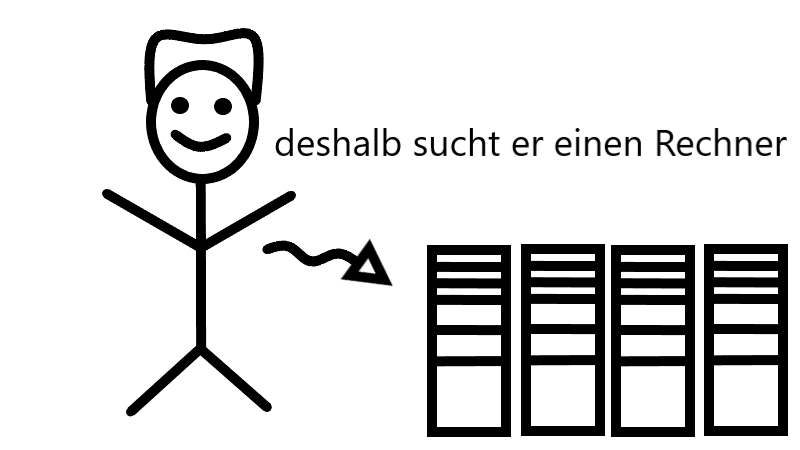
\includegraphics[width=\linewidth]{Graphiken/Szene4_Rechnerwahl.png}
	}
	\frame{
		\frametitle{Motivation - Ein Beispiel}
		
\includegraphics[width=\linewidth]{Graphiken/Szene5_Anmelden_Enie.png}
	}
	\frame{
		\frametitle{Motivation - Ein Beispiel}
		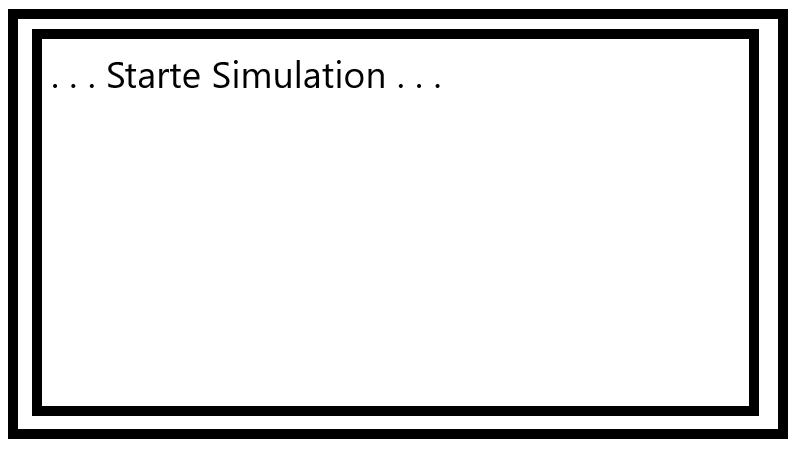
\includegraphics[width=\linewidth]{Graphiken/Szene6_Start_Enie.png}
	}
	\frame{
		\frametitle{Motivation - Ein Beispiel}
		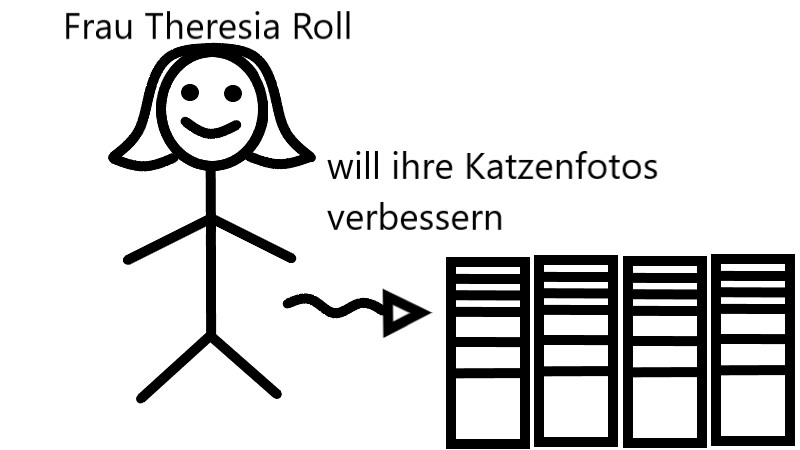
\includegraphics[width=\linewidth]{Graphiken/Szene7_FrauTheresiaRoll.png}
	}
	\frame{
		\frametitle{Motivation - Ein Beispiel}
		
\includegraphics[width=\linewidth]{Graphiken/Szene8_Anmelden_Roll.png}
	}
	\frame{
		\frametitle{Motivation - Ein Beispiel}
		
\includegraphics[width=\linewidth]{Graphiken/Szene9_Last.png}
	}
	\frame{
		\frametitle{Motivation - Ein Beispiel}
		
\includegraphics[width=\linewidth]{Graphiken/Szene10_Enie_merkt.png}
	}
	\frame{
		\frametitle{Motivation - Ein Beispiel}
		
\includegraphics[width=\linewidth]{Graphiken/Szene11_KeineRechenzeit.png}
	}
	\frame{
		\frametitle{Motivation - Ein Beispiel}
		
\includegraphics[width=\linewidth]{Graphiken/Szene12_Trauer.png}
	}
	\frame{
	    \frametitle{Die Lösung: Balanced Banana}
	    \begin{itemize}
	    \item Schluss damit: Aufgaben automatisiert und priorisiert verteilen.\pause
	    \item Bei Balanced Banana werden Aufgaben mit nur einem Befehl gestartet.\pause
	    \item Balanced Banana übernimmt den Rest: Nimmt die Aufgabe und tut sie auf den Arbeiter.\pause
	    \item Balanced Banana respektiert Prioritäten.\pause
	    \item Somit wird Herr G.Enies hochpriorisierte Simulation stets Frau I.D.Iots unwichtigen Katzenbildern vorgezogen.
	    \end{itemize}
	}
	\frame{
		\frametitle{Balanced Banana: Die sehr guten Funktionen}
		\begin{itemize}
		\item \textbf{Automatische Verteilung} Lästige Verbindungen mit anderen Rechnern gehören der Vergangenheit an.\pause
		\item \textbf{Prioritäten} Das Wichtigste kommt immer zuerst.\pause
		\item \textbf{Pausen} Aufgaben auf Wunsch pausieren oder ein Backup erstellen.\pause
		\item \textbf{Statistiken} Alle Informationen zum Status der Aufgaben auf einen Blick.
		\end{itemize}
	}
\end{document}